%\documentclass[12pt]{report}
%\setlength{\parindent}{0mm}
%\setlength{\parskip}{14pt}
%\renewcommand{\baselinestretch}{2.0}
%\setlength{\topmargin}{0pt}
%\setlength{\headheight}{0pt}
%\setlength{\headsep}{0pt}
%\setlength{\footskip}{45pt}
%\setlength{\textwidth}{465pt}
%\setlength{\textheight}{660pt}
%\setlength{\oddsidemargin}{10pt}
%\newcommand{\RR}{\mathrm{I\!R\!}}
%\newcommand{\FF}{\mathrm{I\!F\!}}
%\newcommand{\dt}{\frac{\partial}{\partial t}}
%\newcommand{\Dt}{\frac{D}{Dt}}
\newtheorem{defi}{Definition}[chapter]
%\newtheorem{theo}{Theorem}[chapter]

%\begin{document}

\chapter{Derivation of Navier-Stokes Equations}

In this chapter, we obtain Navier-Stokes Equations from the conservation of mass and linear momentum. The main ingredient in our derivation is Reynold's transport theorem. The latter is a generalization of the classical Leibniz formula. It permits the computation of the time rate of change of an integral on a time-dependent domain. The analysis preceding the derivation of the Navier-Stokes equations relies on the lecture notes by Mason \cite{feln,fmln}. 

\section{Reynold's transport theorem}

Consider a fluid body which is composed of a set of particles. At each instant $t$, the particles are assigned a unique point in a closed and bounded region ${\cal B }_{t}$ of the three-dimensional Euclidean space. Each point of ${\cal B }_{t}$ is occupied by only one particle.

\begin{defi}
${\cal B }_{t}$ is called the \textbf{configuration} of the body at time $t$.
\end{defi} 

The configuration at time $t=0$ is usually chosen as the reference configuration and denoted by ${\cal B }_{0}$. Let $\textbf{X} = (X_{1},X_{2},X_{3})$ be the Cartesian coordinates of a particle in ${\cal B }_{0}$. The motion of the body is described by giving the position $\textbf{x}$ of the particle $\textbf{X}$ at time $t$.

Let $ \chi : \Omega_{1} \times(0,T) \longrightarrow \Omega_{2}$; where $(\textbf{X},t) \longmapsto \textbf{x} = \chi (\textbf{X},t) = (\chi_{1}(X,t),\chi_{2}(X,t),\chi_{3}(X,t)) $ 

$\displaystyle{\chi_{i}, (i = 1,2,3)}$ are differentiable with continuous derivatives.

$\displaystyle{\forall t \in (0,T), \chi (\cdot,t) : \Omega_{1} \longrightarrow \Omega_{2}}$ is a diffeomorphism.

\begin{defi}
The mapping $\chi$ from the initial configuration to the final configuration is called a \textbf{deformation} of the body.
\end{defi}

The coordinates of the point $\textbf{X}$, denoted by $(X_1, X_2, X_3)$ are called material(Lagrangian) coordinates. 

The coordinates of the point $\textbf{x}$, denoted by $(x_1, x_2, x_3)$ are called spatial(Eulerian) coordinates.

Figure (\ref{DB}) illustrates the deformation of a body from its undeformed configuration to its deformed configuration.
\begin{figure}
\begin{center}
\caption{Deformation of the Body}
\label{DB}
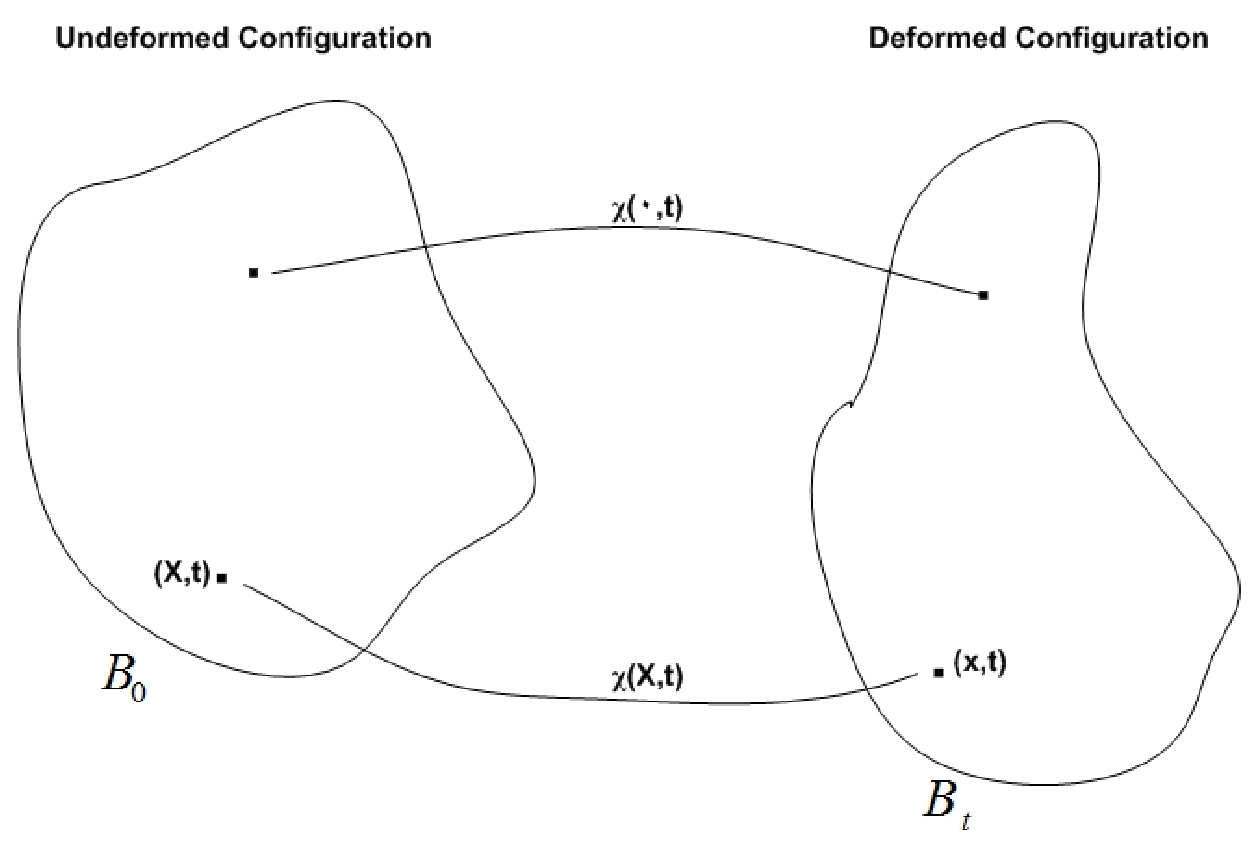
\includegraphics[scale = .5]{config_gragh_marvin.eps}
\end{center}
\end{figure}

We shall adopt the following notations:\\
Capital letters A,B,C\ldots as indices refer to material coordinates: $ X_{A},\  A \in \left\{1,2,3\right\}$\\
Lowercase letters i,j,k\ldots as indices refer to spatial coordinates: $ x_{i},\  i \in \left\{1,2,3\right\}$\\
Eienstein's summation convention:\\
$$ x_{i}x_{i} = x_{1}^2 + x_{2}^2 + x_{3}^2 $$
$$ X_{A}X_{A} = X_{1}^2 + X_{2}^2 + X_{3}^2 $$

\begin{defi}
The \textbf{velocity} of the particle $X$ denoted $\dot x$ is defined by
\begin{equation}
\label{ch1:t1}
 \textbf{v} = \dot x = \frac{\partial \chi(X,t)}{\partial t}
  \end{equation}
\end{defi}

\begin{defi}
The \textbf{acceleration} of the particle $X$ denoted $\ddot x$ is defined by
\begin{equation}
\label{ch1:t2}
\dot \textbf{v} = \ddot x = \frac{\partial^2 \chi(X,t)}{\partial t^2}
\end{equation}
\end{defi}

A quantity can be expressed as a function of either the Lagrangian description $(\textbf{X},t)$ or the Eulerian description $(\textbf{x},t)$.
Changing from one description to the other can be done by using

$$ \Psi(\chi^{-1}(\textbf{x},t),t) = \psi(\textbf{x},t) $$
or
$$ \psi(\chi(\textbf{X},t),t) = \Psi(\textbf{X},t) $$

\begin{defi}
\begin{em} 
The \textbf{alternating tensor}, denoted as $\epsilon_{ABC}$, is defined by 
\begin{equation}
\epsilon_{ABC} = \left\{ 
\begin{array}{l r}
1 & \mbox{if $(A B C)$ is an even permutation of $\{1,2,3\}$}\\
-1 & \mbox{if $(A B C)$ is an odd permutation of $\{1,2,3\}$}\\
0 & \mbox{otherwise}
\end{array}
\right.
\end{equation}  
\end{em}
\end{defi}

\begin{defi}
The \textbf{deformation gradient} denoted $F_{\chi}$ is defined by
\begin{equation}
\label{ch1:t3}
 F_{\chi} = x_{i,A} = \left[\frac{\partial \chi_{i}}{\partial X_{A}}\right] i,A \in \left\{1,2,3\right\}
  \end{equation}
\end{defi}

The deformation gradient of the map $\chi$ is non-singular, since $\chi$ is invertible, and its Jacobian is defined as $J_{\chi} = \mbox{det}F_{\chi}$.

The meaning of $J_{\chi}$  as the change in volume due to the change of coordinates $\chi$ can be easily understood from the following theorem.

\begin{theo}
\begin{em}
Let $dV$ be an infinitesimal domain, given by the triple product $dV = dx^{(1)} \cdot ( dx^{(2)} \times dx^{(3)})$. Also let $dV_{0} = dX^{(1)} \cdot ( dX^{(2)} \times dX^{(3)})$ be the push forward of $dV$, that is $dx^{(i)} = F_{\chi}dX^{(i)}$, for $i\in\left\{1,2,3\right\}$. Then, $$ dV = J_{\chi}dV_{0}.$$
\end{em}
\end{theo}


\textbf{Proof.} $$ dx_{i}^{(\alpha)} = x_{i,A}\ dX_{A}^{(\alpha)} $$
Thus \begin{eqnarray*} \mbox{det}[dx_{i}^{(\alpha)}] &=& \mbox{det}[x_{i,A}\ dX_{A}^{(\alpha)}]\\ \\
&=& \mbox{det}[x_{i,A}]\  \mbox{det}[dX_{A}^{(\alpha)}]\\ \\
&=& J_{\chi} \mbox{det}[dX_{A}^{(\alpha)}]
\end{eqnarray*}
But,
\begin{eqnarray*} \mbox{det}[dx_{i}^{(\alpha)}] &=& \epsilon_{ijk}dx_{i}^{(1)}dx_{j}^{(2)}dx_{k}^{(3)}\\ \\
&=& dx_{i}^{(1)}\epsilon_{ijk} \ dx_{j}^{(2)}dx_{k}^{(3)}\\ \\
&=& dX^{(1)} \cdot ( dX^{(2)} \times dX^{(3)})
\end{eqnarray*}
Therefore,
$$ d\stackrel{\rightarrow}{x} = J_{\chi}d\stackrel{\rightarrow}{X}.$$

which concludes the proof.


\begin{theo}
$$ \frac{DJ_{\chi}}{Dt} = J_{\chi}\mbox{div}(v)$$
\end{theo}

\textbf{Proof.}
$$ J_{\chi} = \mbox{det}[x_{i,A}] = \epsilon_{ABC}\ x_{1,A}\ x_{2,B}\ x_{3,C} $$
Thus
$$ \frac{DJ_{\chi}}{Dt} = \epsilon_{ABC}[(\frac{D}{Dt}x_{1,A})\ x_{2,B}\ x_{3,C} + x_{1,A}\ (\frac{D}{Dt})x_{2,B}\ x_{3,C} + x_{1,A}\ x_{2,B}\ (\frac{D}{Dt})x_{3,C}]$$
But,
\begin{eqnarray*} \frac{D}{Dt}x_{1,A} &=& \frac{\partial^2}{\partial t \partial X_{A}}x_{1}(X,t)\\
&=& \frac{\partial^2}{\partial X_{A} \partial t }x_{1}(X,t)\\ 
&=& \frac{\partial v_{1}}{\partial X_{A}}\\
&=& \frac{\partial v_{1}}{\partial x_{k}} \frac{\partial x_{k}}{\partial X_{A}}\\
&=& v_{i,k} \frac{\partial x_{k}}{\partial X_{A}}
\end{eqnarray*}
Thus 
\begin{eqnarray*} \epsilon_{ABC}(\frac{D}{Dt}x_{1,A}) x_{2,B} x_{3,C} &=& \epsilon_{ABC}v_{1,k}\ x_{k,A}\ x_{2,B}\ x_{3,C}\\
&=& v_{1,1} \epsilon_{ABC}x_{1,A})\ x_{2,B}\ x_{3,C}\\
&=& v_{1,1}J_{\chi}
\end{eqnarray*}
Similarly, 
$$ \epsilon_{ABC} x_{1,A} \ (\frac{D}{Dt})x_{2,B}) x_{3,C} = v_{2,2}J_{\chi} $$
and
$$ \epsilon_{ABC} x_{1,A} x_{2,B} (\frac{D}{Dt})x_{3,C} = v_{3,3}J_{\chi} $$
Thus 
\begin{eqnarray*}\frac{DJ_{\chi}}{Dt} &=& v_{k,k}J_{\chi}\\ 
&=& J_{\chi}\mbox{div}(v)
\end{eqnarray*}




\begin{theo}
Let $V$ be a subset of the deformed configuration, and let $V_{0}$ be a subset of the undeformed configuration. Then for a differentiable function $f$ with continuous partial derivatives, we have
\begin{equation}
\frac{D}{Dt} \int_{V} f(\stackrel{\rightarrow}{x},t)dV = \int_{V}\left\{ {\frac{\partial f}{\partial t} + \nabla\cdot(f\stackrel{\rightarrow}{u})}\right\}dV
\end{equation}
\end{theo}

\textbf{Proof.}
\begin{eqnarray*}
 \frac{D}{Dt} \int_{V} f(\stackrel{\rightarrow}{x},t)dV &=& \frac{D}{Dt} \int_{V_{0}} f(\chi(\textbf{X},t),t)J_{\chi}dV_{0}\\ \\
 &=& \int_{V_{0}}\left\{\frac{Df(\chi(\textbf{X},t),t)}{Dt}J_{\chi} + f(\chi(\textbf{X},t),t)\frac{DJ_{\chi}}{Dt}\right\}dV_{0}\\ \\ 
 &=& \int_{V_{0}}\left\{\frac{Df(\chi(\textbf{X},t),t)}{Dt}J_{\chi} + f(\chi(\textbf{X},t),t)J_{\chi}\nabla v\right\}dV_{0}\\ \\
 &=& \int_{V_{0}}\left\{\frac{Df(\chi(\textbf{X},t),t)}{Dt} + f(\chi(\textbf{X},t),t)\nabla v\right\}J_{\chi}dV_{0}\\ \\
 &=& \int_{V_{0}}\left\{\frac{\partial f(\chi(\textbf{X},t),t)}{\partial t} + v\cdot \nabla f(\chi(\textbf{X},t),t) + f(\chi(\textbf{X},t),t)\cdot \nabla v\right\}J_{\chi}dV_{0}\\ \\
 &=& \int_{V}\left\{\frac{\partial f(\stackrel{\rightarrow}{x},t)}{\partial t} + \mbox{div}(f(\stackrel{\rightarrow}{x},t)v)\right\}dV\\ \\
 \end{eqnarray*}

The Dominated Convergence Theorem is what allows for the passing of the material derivative inside of the integral operator.


\section{Conservation of Mass}


The mass of a fluid $(M_{fluid})$ is given by the integral of the fluid density over the fluid domain i.e. \begin{equation} M_{fluid} = \int_{V} \rho(\stackrel{\rightarrow}{x},t)dV \end{equation}
The Conservation of Mass principle states that the derivative of mass w.r.t time must vanish i.e. \begin{equation} \frac{D}{Dt} \int_{V} \rho(\stackrel{\rightarrow}{x},t)dV = 0. \end{equation}
Applying Reynold's Transport Theorem, we have \begin{equation} \frac{D}{Dt} \int_{V} \rho(\stackrel{\rightarrow}{x},t)dV = \int_{V} \left\{\frac{\partial \rho}{\partial t} + \nabla \cdot(\rho \stackrel{\rightarrow}{u})\right\}dV = 0. \end{equation} Since we are working within the confines of the continuum hypothesis and since this equation must hold true for arbitrarily small domains, we can infer that \begin{equation}\label{cce} \frac{\partial \rho}{\partial t} + \nabla \cdot(\rho \stackrel{\rightarrow}{u}) = 0.\end{equation} which is the continuity equation for compressible flows.

Expanding the divergence term in Eq. (\ref{cce}) yields \begin{equation} \frac{D\rho}{Dt} + \rho \nabla \cdot \stackrel{\rightarrow}{u} = 0. \end{equation} where $\displaystyle{ \frac{D}{Dt} = \frac{\partial}{\partial t} + (\stackrel{\rightarrow}{u}\cdot \nabla)} $

In the case where the density remains constant, Eq.(\ref{cce}) simplifies to \begin{equation}\label{ice} \nabla \cdot \stackrel{\rightarrow}{u} = 0 \end{equation} which is the continuity equation for incompressible flows.

\section{Conservation of Momentum}

The Conservation of Linear Momentum Principle states that the rate of change of momentum w.r.t time is equal to the sum of the acting forces. This is given mathematically by 
\begin{equation}
\frac{D}{Dt}\int_{V} \rho(\stackrel{\rightarrow}{x},t) \stackrel{\rightarrow}{u}dV = \sum \mbox{acting forces}
\end{equation}
 The forces of interest are body forces such as gravity, Coriolis force etc. and surface forces such as pressure and internal friction(viscosity).

Body forces will be expressed as \begin{equation} \int_{V} \rho(\stackrel{\rightarrow}{x},t) g(\stackrel{\rightarrow}{x},t)dV \end{equation} and surface forces will be expressed as \begin{equation} \int_{\partial V} \sigma(\stackrel{\rightarrow}{x},t)\stackrel{\rightarrow}{n}ds \end{equation}
where $\sigma$ is the stress tensor, $\stackrel{\rightarrow}{n}$ is the outward unit normal, and $ \partial V $ is the boundary of the domain $V$

Recasting Newton's 2nd law with the aforementioned information in mind, we have \begin{equation} \frac{D}{Dt} \int_{V} \rho(\stackrel{\rightarrow}{x},t) \stackrel{\rightarrow}{u}dV = \int_{V} \rho(\stackrel{\rightarrow}{x},t) g(\stackrel{\rightarrow}{x},t)dV + \int_{\partial V} \sigma(\stackrel{\rightarrow}{x},t)\stackrel{\rightarrow}{n}ds \end{equation}

Applying Reynold's Transport Theorem to the term on the left yields \begin{equation} \int_{V} \left\{\frac{\partial \rho \stackrel{\rightarrow}{u}}{\partial t} + \nabla \cdot \rho \stackrel{\rightarrow}{u}\stackrel{\rightarrow}{u}\right\}dV = \int_{V} \rho(\stackrel{\rightarrow}{x},t) g(\stackrel{\rightarrow}{x},t)dV + \int_{\partial V} \sigma(\stackrel{\rightarrow}{x},t)\stackrel{\rightarrow}{n}ds \end{equation}
After applying the Divergence Theorem to the last term and regrouping the equation we arrive at \begin{equation} \label{cmom}\frac{\partial \rho \stackrel{\rightarrow}{u}}{\partial t} + (\stackrel{\rightarrow}{u} \cdot \nabla)\rho\stackrel{\rightarrow}{u} + \rho\stackrel{\rightarrow}{u}\nabla \cdot \stackrel{\rightarrow}{u} - \rho \stackrel{\rightarrow}{g} - \nabla \cdot \sigma = 0 \end{equation}

The stress tensor $\sigma$ for viscous fluids is defined as \begin{equation} \sigma := -pI + \tau := -p + \lambda \mbox{div}(\stackrel{\rightarrow}{u})I + 2\mu\delta. \end{equation} Using this stress tensor in Eq. (\ref{cmom}), yields \begin{equation}\label{cmoms} \frac{\partial \rho \stackrel{\rightarrow}{u}}{\partial t} + (\stackrel{\rightarrow}{u} \cdot \nabla)\rho\stackrel{\rightarrow}{u} + \rho\stackrel{\rightarrow}{u}\nabla \cdot \stackrel{\rightarrow}{u} + \mbox{grad}p = (\mu + \lambda)\mbox{grad}(\mbox{div}(\stackrel{\rightarrow}{u})) + \mu\Delta\stackrel{\rightarrow}{u} + \rho\stackrel{\rightarrow}{g} \end{equation}

If the fluid being studied is incompressible(i.e $\rho$ = $\rho_{\infty}$ = constant), Eq. (\ref{cmoms}) reduces to \begin{equation} \label{imom}\frac{\partial \stackrel{\rightarrow}{u}}{\partial t} + (\stackrel{\rightarrow}{u} \cdot \nabla)\ \stackrel{\rightarrow}{u} + \frac{1}{\rho_{\infty}}\mbox{grad}p = \frac{\mu}{\rho_{\infty}}\Delta\stackrel{\rightarrow}{u} + \stackrel{\rightarrow}{g} \end{equation}

Equation (\ref{ice}) together with Eq.(\ref{imom}) comprise what is today known as the Navier-Stokes Equations for incompressible flows.

\section{Dimensional Analysis}

Performing experiments for flow applications can be very expensive and time consuming. Take for example studying the flow of air around automobiles. One would need to build the automobile as well as reproduce the conditions under which they operate. As we know, this is more easily said than done. These kinds of applications motivated the need for prototypes and models. The first step in this process is to nondimensionalize the governing equations. This is done by selecting reference quantities for each of the variable present in the equation. Those variable are $\stackrel{\rightarrow}{u}$,$\stackrel{\rightarrow}{x}$,$p$,and $t$ and the associated reference quantities are $V$,$L$,$\rho_{\infty}V^2$, and $\displaystyle{\frac{L}{V}}$. A quick check will show that these variables and their associated reference quantities are dimensionally homogeneous. Because of this, the dimensionless quantities can be defined as \begin{equation} \stackrel{\rightarrow}{u}^* := \frac{\stackrel{\rightarrow}{u}}{V}, \stackrel{\rightarrow}{x}^* := \frac{\stackrel{\rightarrow}{x}}{L}, p^* := \frac{p}{\rho_{\infty}V^2}, t^* := \frac{Vt}{L} \end{equation}

Recasting equation (15) with these new variable yields, \begin{equation} \frac{V^2}{L}\frac{\partial \stackrel{\rightarrow}{u}^*}{\partial t^*} + \frac{V^2}{L}(\stackrel{\rightarrow}{u}^* \cdot \mbox{grad}^*)\stackrel{\rightarrow}{u}^* + \frac{V^2}{L}\mbox{grad}^* p^* = \frac{V\mu}{L{^2}\rho_{\infty}} \Delta^* \stackrel{\rightarrow}{u}^* + \stackrel{\rightarrow}{g} \end{equation}

Multiplying through by $\displaystyle{\frac{L}{V^2}}$ yields, \begin{equation} \frac{\partial \stackrel{\rightarrow}{u}^*}{\partial t^*} + (\stackrel{\rightarrow}{u}^* \cdot \mbox{grad}^*)\stackrel{\rightarrow}{u}^* + \mbox{grad}^* p^* = \frac{\mu}{L\rho_{\infty}V} \Delta^* \stackrel{\rightarrow}{u}^* + \frac{L}{V^2} \stackrel{\rightarrow}{g} \end{equation}

With the introduction of the dimensionless body force \begin{equation} \stackrel{\rightarrow}{g^{*}} := \frac{L \stackrel{\rightarrow}{g}}{V^2} = \frac{1}{Fr^2}\frac{\stackrel{\rightarrow}{g}}{\left\|\stackrel{\rightarrow}{g}\right\|} \end{equation} the equation becomes \begin{equation} \label{dmome}\frac{\partial \stackrel{\rightarrow}{u}^*}{\partial t^*} + (\stackrel{\rightarrow}{u}^* \cdot \mbox{grad}^*)\stackrel{\rightarrow}{u}^* + \mbox{grad}^* p^* = \frac{\mu}{L\rho_{\infty}V} \Delta^* \stackrel{\rightarrow}{u}^* + \stackrel{\rightarrow}{g^{*}} \end{equation}

The coefficient of the Laplacian gives the reciprocal of the Reynolds number and the last term involves the reciprocal of the square of the Froude number. Recasting Eq. (\ref{dmome}) with this in mind and dropping the * for  convenience yields, \begin{equation} \frac{\partial \stackrel{\rightarrow}{u}}{\partial t} + (\stackrel{\rightarrow}{u} \cdot \mbox{grad})\stackrel{\rightarrow}{u} + \mbox{grad} p = \frac{1}{Re} \Delta \stackrel{\rightarrow}{u} + \stackrel{\rightarrow}{g} \end{equation}

Doing this for the continuity equation will leave it unchanged. It is worth mentioning that the dimensionless quantities that arise in this equation depend heavily on the the reference quantities which usually depend on what is of interest in the flow being analyzed \cite{ffm}. 

\section{Geometries and Boundary Conditions}

As stated previously, the Navier-Stokes Equations are the governing equations for fluid flow. Having this in mind, a question that might arise quite naturally is how does one obtain different flow fields as it relates to various applications. The answer to this question resides in the fact that a specific geometry and various boundary conditions must be supplied when using the Navier-Stokes Equations for a particular application. The boundary conditions that are of particular interest are the Dirichlet boundary condition(no-slip boundary condition), Neumann boundary conditions, mixed boundary conditions, and periodic boundary conditions. Let $\varphi_{n}$ denote the component of velocity orthogonal to the boundary in the exterior normal direction, $\varphi_{t}$ the component of velocity parallel to the boundary in the tangential direction, and $ \displaystyle{\frac{\partial \varphi_{n}}{\partial n}}$ and $ \displaystyle{\frac{\partial \varphi_{t}}{\partial n}}$ be their respective derivatives in the normal direction. 

\subsection{Dirichlet Boundary Condition}

Dirichlet boundary conditions specify the values a solution must take on the boundary of the domain. In the case of fluid flow problems, the no-slip conditions, which are homogeneous Dirichlet boundary conditions, are often enforced on the boundaries of the given geometry. The no-slip condition says that no fluid penetrates the boundary and the fluid is at rest there. Mathematically, this given by \begin{equation} \varphi_{n} = 0, \ \ \ \ \ \  \varphi_{t} = 0 \end{equation} These are to be understood irrespective of the boundary being investigated.

\subsection{Neumann Boundary Condition}

Neumann boundary conditions specify the values that the directional derivative must satisfy along the outward normal to the boundary of the domain. A situation where this occurs is when outflow conditions, which are homogenous Neumann boundary conditions, are supplied. They state that neither velocity component changes in the direction normal to the boundary. Mathematically, this is given by \begin{equation} \frac{\partial \varphi_{n}}{\partial n} = 0, \ \ \ \ \ \ \frac{\partial \varphi_{t}}{\partial n} = 0. \end{equation} The partial derivatives are taken with respect to different axes depending on the orientation of the boundaries.

\subsection{Mixed Boundary Condition}

Mixed boundary conditions are combinations of Dirichlet and Neumann boundary conditions. A situation where this occurs is when free-slip conditions, which are homogeneous mixed boundary conditions, are supplied. They state that no fluid penetrates the boundary and there are no frictional losses at the boundary. Mathematically, this is given by \begin{equation} \varphi_{n} = 0, \ \ \ \ \ \ \frac{\partial \varphi_{t}}{\partial n} = 0 \end{equation}

\subsection{Periodic Boundary Condition}

Periodic boundary conditions occur when the flow problem is periodic over one or more of the coordinate directions. A situation where this occurs is flow over an undulating surface. Since the values on the boundaries are repeated over some period $a$, the computations can be restricted to one period interval.

\section{Conclusion}

In this chapter, we presented the derivation of the Navier-Stokes equations from the conservation of mass and linear momentum. In order to do this, we use Reynold's Transport Theorem. Following the derivation, dimensional analysis of the equations is presented and boundary conditions are discussed so that we have a well-posed problem to work with. In the next chapter, we move from the continuous problem to the discrete problem.
%
%\end{document}